% !TEX root = ./main.tex

To assess how the filtered stepper supports instructors and students
learning functional programming, we deployed it in an upper-level
university programming languages course. We first report on the
instructor's experience using the stepper in lecture, then on student
usage and survey responses from homework assignments.

\subsection{Lecture Integration}

Before the filtered stepper was integrated into Hazel, the instructor
of the course presented small-step reductions in lecture by hand,
working through example traces on the whiteboard. This required significant
time writing out reductions that were mostly similar between steps.
Since the stepper was deployed, the instructor has
used it to run these example evaluations live in lecture instead.
This shift had three practical effects. First, walking through an
evaluation became substantially less tedious. Filter annotations
let the instructor collapse routine reductions and surface only the
steps that matter for the lesson at hand, without having to commit
to those choices in slide content ahead of time. Second, when a
student asked a follow-up question, the instructor was able to edit the
example and rerun the stepper in real time. With hand-worked paper
traces, exploring a ``what if we changed this?'' would have stalled
the lecture. Third, the
stepper served as a running demonstration of Hazel itself: the same
environment the students were using for their assignments was on
display in lecture, with its hole-driven editor, live evaluation,
and stepper visible side by side.

\subsection{Assignment Integration}

The assignments we evaluated our stepper on usually consist of several tasks, each of which asks students to implement or complete a function to pass given unit tests. To help students focus on their task, we provide prelude Hazel definitions that they can use directly in their assignments. We do not want students to inspect the evaluation of the prelude, as this would break the narrative that the prelude already exists in the environment. We therefore insert a \lstinline[language=hazel]{debug hide($e)} at the very top of the program, and a \lstinline[language=hazel]{debug stop($e)} before the user program. Whenever the user turns the stepper on, it skips evaluation of the prelude and stops at the entrance of the user program.

We collected anonymous data from students during one of their
assignments. The number of steps used by students is shown in
Figure~\ref{fig:eval-num-steps}.

\begin{figure}[ht]
  \centering
  \begin{minipage}{.40\linewidth}
    \begin{subfigure}{\linewidth}
      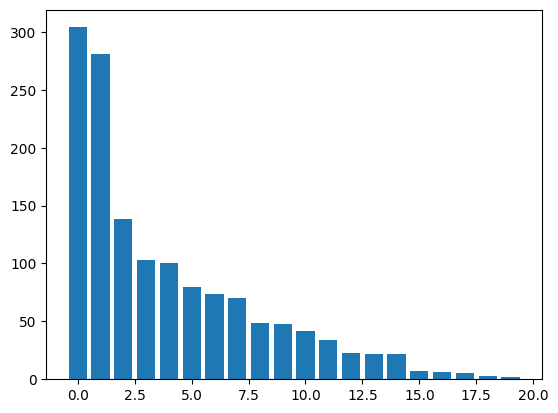
\includegraphics[width=\textwidth]{images/data-steps-2024-w24-a1.png}
      \caption{Winter 2024, sample size 33}
      \label{fig:eval-num-steps-w24}
    \end{subfigure}
  \end{minipage}
  \quad
  \begin{minipage}{.40\linewidth}
    \begin{subfigure}{\linewidth}
      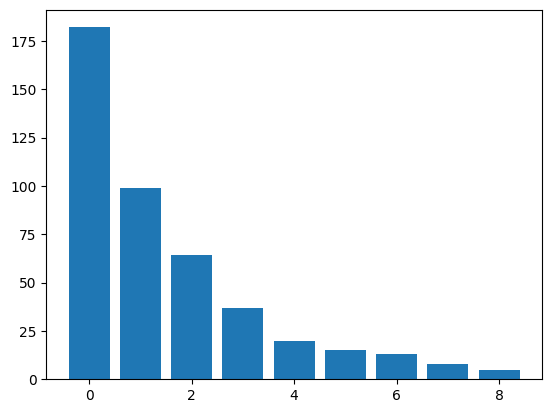
\includegraphics[width=\textwidth]{images/data-steps-2024-f24-a1.png}
      \caption{Fall 2024, sample size 20}
      \label{fig:eval-num-steps-f24}
    \end{subfigure}
  \end{minipage}
  \caption{Number of steps used by students}
  \label{fig:eval-num-steps}
\end{figure}

Students were never explicitly instructed in how to use the stepper,
and were not asked to use it on the homework. Even so, nearly half
of them saw the instructor demonstrate it in lecture and chose to
use it themselves on the assignment.

The number of steps used by students roughly conforms to an
exponential distribution. A small portion of students use the
stepper extensively.

To complement the usage data, we administered an anonymous end-of-term
survey to the same cohort. Of 25 respondents, 20 reported using the
stepper and 12 of those adopted at least one of the
\lstinline[language=hazel]{hide}, \lstinline[language=hazel]{stop},
\lstinline[language=hazel]{eval}, or \lstinline[language=hazel]{step}
filter keywords. The Likert responses are summarized in
Table~\ref{tab:eval-survey-likert}. We classify usage using the direct
usage question and summarize Likert responses only for respondents who
reported using the stepper.

\begin{table}[ht]
  \centering
  \caption{Self-reported experience with the stepper among users, Strongly/Somewhat collapsed ($n=20$).}
  \label{tab:eval-survey-likert}
  \begin{tabular}{lccc}
    \toprule
    Statement (paraphrased) & Agree & Neither & Disagree \\
    \midrule
    Difficult to read                       & 5  & 4 & 11 \\
    Surprised by green highlighting         & 9  & 7 & 4  \\
    Helped identify or correct bugs         & 12 & 5 & 3  \\
    Helped understand Hazel's features      & 13 & 6 & 1  \\
    Long and tedious to interact with       & 7  & 5 & 8  \\
    \bottomrule
  \end{tabular}
\end{table}

Three observations triangulate with the usage data. First, the
strongest positive response (13 vs.\ 1) is for \emph{understanding}
language features rather than bug-finding (12 vs.\ 3), and the
free-text ``what did you use it for?'' question agrees: ``understanding
how Hazel evaluates'' is mentioned slightly more often than
``debugging,'' consistent with the stepper's substitution-based,
source-level design. Second, readability is not the issue (11 vs.\ 5),
but ``long and tedious'' splits evenly (7 vs.\ 8) and tracks the
long-tailed shape of Figure~\ref{fig:eval-num-steps}; the
12-of-20 adoption rate of the filter keywords suggests students
reach for filters as friction reduction, as designed. Third, the
green-highlighting question drew nearly half the users to agree
(9 of 20), indicating that the lexical scoping of filters is not
self-evident in the current source-text-only interface, motivation
for the graphical filter panel discussed as future work.

The survey is small ($n=25$), single-cohort, voluntary, and
self-report. One respondent reported uniformly negative experiences
attributed to bugs in the deployed prototype.

%%% Local Variables:
%%% mode: LaTeX
%%% TeX-master: "main"
%%% End:
